\documentclass{article}
\def\Rfunc#1{\textbf{#1()}}
\usepackage{graphicx}
\usepackage{fullpage}
\usepackage{times}
\usepackage{hyperref}

\title{Assignment 2}

\author{Sta242 Winter 2015 \\
Duncan Temple Lang
}
\begin{document}
\maketitle
\begin{center}
\textbf{Due}: Wednesday, 29th April, 4pm \\
\textbf{Send electronic version (PDF and R package in separate files) and the address of the git
  repository to \texttt{dtemplelang@ucdavis.edu} with the \textbf{exact} subject \textbf{STA242 Assignment 2}}\\
\textbf{Put a printed copy of the PDF and the code in Nick's mailbox.}
\end{center}

This project involves a simulation of a 
simple traffic flow model that exhibits a phase transition.

This homework focuses on several programming topics.  One is writing
\textit{good}, flexible, reusable R functions and testing them to
verify they are correct.  The second topic is to use the S3 class
mechanism to define classes and methods for printing and plotting
objects representing the simulation.  
The third element is to make the code efficient, e.g., by profiling and using different
computational approaches.
The final aspect is to create an
R package containing your code, help files and anything else.
This will involve
\begin{enumerate}
\item Writing Functions,
\item Testing Functions,
\item Debugging,
\item Vectorized computations (rather than loops, if possible),
\item Profiling,
\item S3 classes and methods,
\item R packages.
\end{enumerate}


You are to use git for the assignment to manage the code.


\section{The Simulation Process}

The simulation is about cars moving on a grid.  We have two types of
cars, ``blue'' and ``red''.  These move on a two-dimensional grid of
size $r$ by $c$.  We populate the grid by placing $\rho \times r
\times c$ (with $0 < \rho < 1$) cars at random positions in the $r
\times c$ cells, but with no two cars occupying the same cell.  The
type of each car is selected randomly from ``red'' and ``blue'' with
equal probability.  ( You can explore different probabilities, or
forcing the numbers to be the same.)

Now the cars can move.  In our configuration, the blue cars move at
time periods $t = 1, 3, 5, ...$ and the red cars move at time periods
$t = 2, 4, 6, ...$, i.e., they alternate in time.  The ``blue'' cars move
vertically upward.  The ``red'' cars move horizontally rightwards.
When a car gets to the edge of the grid, it ``wraps'' around,
i.e., when a blue car gets to the top row, the next time it moves it goes to the bottom
row of the same column. Similarly a red car that gets to the right edge of the grid will move
next to the first column of the grid, i.e., the extreme left.

A car cannot move to cell if that cells is already occupied by another
car (of any color).

This process is called the Biham-Middleton-Levine Traffic Model and is
of interest because it is one of the very simplest processes that
exhibits a phase-transition, and also self-organizing behavior.  As $\rho$ changes from $.2$ to $.5$,
there is a point at which the behavior dramatically shifts. And recent
research has identified sub-structures.  Additionally, 
while each car has a simple rule to move that only depends on whether another car is in its target
location,  the cars form a collective group and establish a clear pattern of self-organization motion.

\section{Tasks}

\begin{enumerate}

 \item You are to write functions  to simulate this process.
   You want to allow the  caller specify $\rho$ (or the number of cars
   or the number of red and number of blue cars).
   Also, she should be able to specify the dimension of the grid.
  
 \item Your function should return an object with a class to identify it as a BML grid.

 \item You can consider how to represent the state of grid so as to facilitate
   the computations to move the cars in each time step. Different representations
   will lead to different computations which  may be more or less efficient.

 \item Write a \textbf{method} for the function \Rfunc{plot} to
   display the grid. Similarly define a method for \Rfunc{summary} to 
   provide a summary of the current state of the grid.
   One approach for the plot method is to produce something like
  \begin{center}
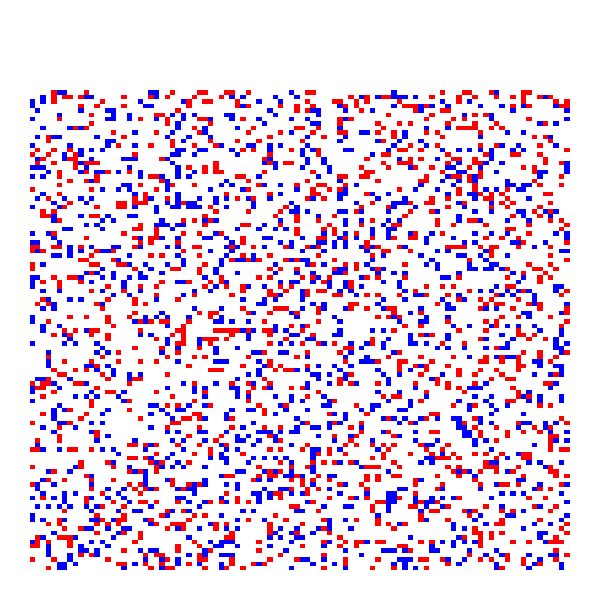
\includegraphics{bmlGrid.pdf}    
  \end{center}
   The functions \Rfunc{image} and \Rfunc{rect} may be useful.

 \item Write one or more functions to move the cars on the grid
 for a time period $t$.
 Verify that it is correct, i.e. do some computations, perhaps write a
 function that compares the new positions with the old.  Make certain
 to test the ``degenerate'' cases.
 

\item Use these functions to simulate the process for different grid sizes
  and values of $\rho$, ranging from $.2$ to $.7$.
  Interpret the results.

\item Time these runs and profile them (using \Rfunc{Rprof} and
  \Rfunc{summaryRprof}) to find where the bottlenecks are occurring.
  Use this information to refine your code or introduce an entirely
  new algorithm/approach (think vectorization!)

 \item Write functions to be able to compute 
   the number of cars that moved, that were blocked,
   and the average velocity at each time step.
   You might want to do this by passing the function(s)
   two grids from time $t$ and $t+1$ respectively and computing
   the quantities from the difference.


 \item Write up your findings both about the stochastic process 
       and also the profiling.  Hand in a PDF file with your writeup
       and an R package.
       Document the primary functions in the package.
       Use \verb+R CMD check+ to verify the package is valid.
   
\end{enumerate}


Your package should make (at least) 2 functions available:
\Rfunc{createBMLGrid} and \Rfunc{runBMLGrid}.
The \Rfunc{createBMLGrid} function should be callable
as
\begin{verbatim}
g = createBMLGrid(r = 100, c = 99, ncars = c(red = 100, blue = 100))
\end{verbatim}
where r and c are the dimensions of the grid and ncars specifies
the number of red and blue cars.

The \Rfunc{rumBMLGrid} should be callable as
\begin{verbatim}
g.out = runBMLGrid(g, numSteps = 10000)
\end{verbatim}
g is the grid (e.g., created with \Rfunc{createBMLGrid})
and numSteps is the number of time steps.

You can make the signatures for these functions richer to accept 
the inputs in richer and more flexible ways, but they must allow
us to call them in the manner shown above.

Take the time to review and refine your functions.  Make certain to
format and comment your code.  Use class inheritance
to customize methods, where appropriate.

Get started on this as soon as possible and ask lots
of questions on Piazza and on the class mailing list.

\textit{
I strongly suggest that you implement a simple version of the code first
and ensure it is working correctly. Then you can optimize it for efficiency.
You will be able to use the correct version as a means of verifying any improved
versions. Include all of the versions in the package.
}


\end{document}
 
% BML
% Boostrap
% Cross-validation and k-nearest neighbor.
% Boostrap
% Graphics
% Reinforced Random walk
% Ad hoc network simulation.
% Fibonacci
